\chapter{Hardware Setup}
\label{ch:hardware_setup}

This chapter details the step-by-step procedures for charging, powering, and physically mounting each hardware component of the system.

\section{Charging the Devices}
All devices (Climber Main, Wristband, Repeater, Base Camp) are powered by internal 18650 Lithium-ion batteries. 

\begin{warningbox}
\textbf{Battery Safety:} Only use the provided USB cables and standard 5V/1A or 5V/2A USB power adapters. Do not expose the devices to extreme heat or puncture the casing, as damaged 18650 batteries pose a severe fire hazard.
\end{warningbox}

\begin{enumerate}
    \item Locate the charging port (Micro-USB or USB-C) on the side of the device enclosure.
    \item Connect the device to a power source.
    \item The charging LED indicator will illuminate \textbf{Red} while charging.
    \item Once fully charged, the indicator will turn \textbf{Green}. Disconnect the charger.
\end{enumerate}

\section{Climber Main Device Setup}

\subsection{Powering On and LED Indicators}
\begin{enumerate}
    \item Press and hold the main power button for 3 seconds.
    \item The RGB LED will undergo a boot sequence (flashing Blue).
    \item \textbf{Solid Blue:} Device is on and waiting for BLE connection.
    \item \textbf{Blinking Green:} GPS lock acquired and LoRa network connected.
    \item \textbf{Flashing Red:} SOS mode activated or critical battery low.
\end{enumerate}

\subsection{Mounting Instructions}
\begin{enumerate}
    \item Use the provided heavy-duty mounting straps.
    \item Secure the Climber Main Device to the \textbf{upper back or shoulder strap} of your backpack.
    \item Ensure the GPS antenna side (marked with a satellite icon) is facing upwards towards the open sky for optimal signal reception.
\end{enumerate}

\begin{figure}[H]
    \centering
    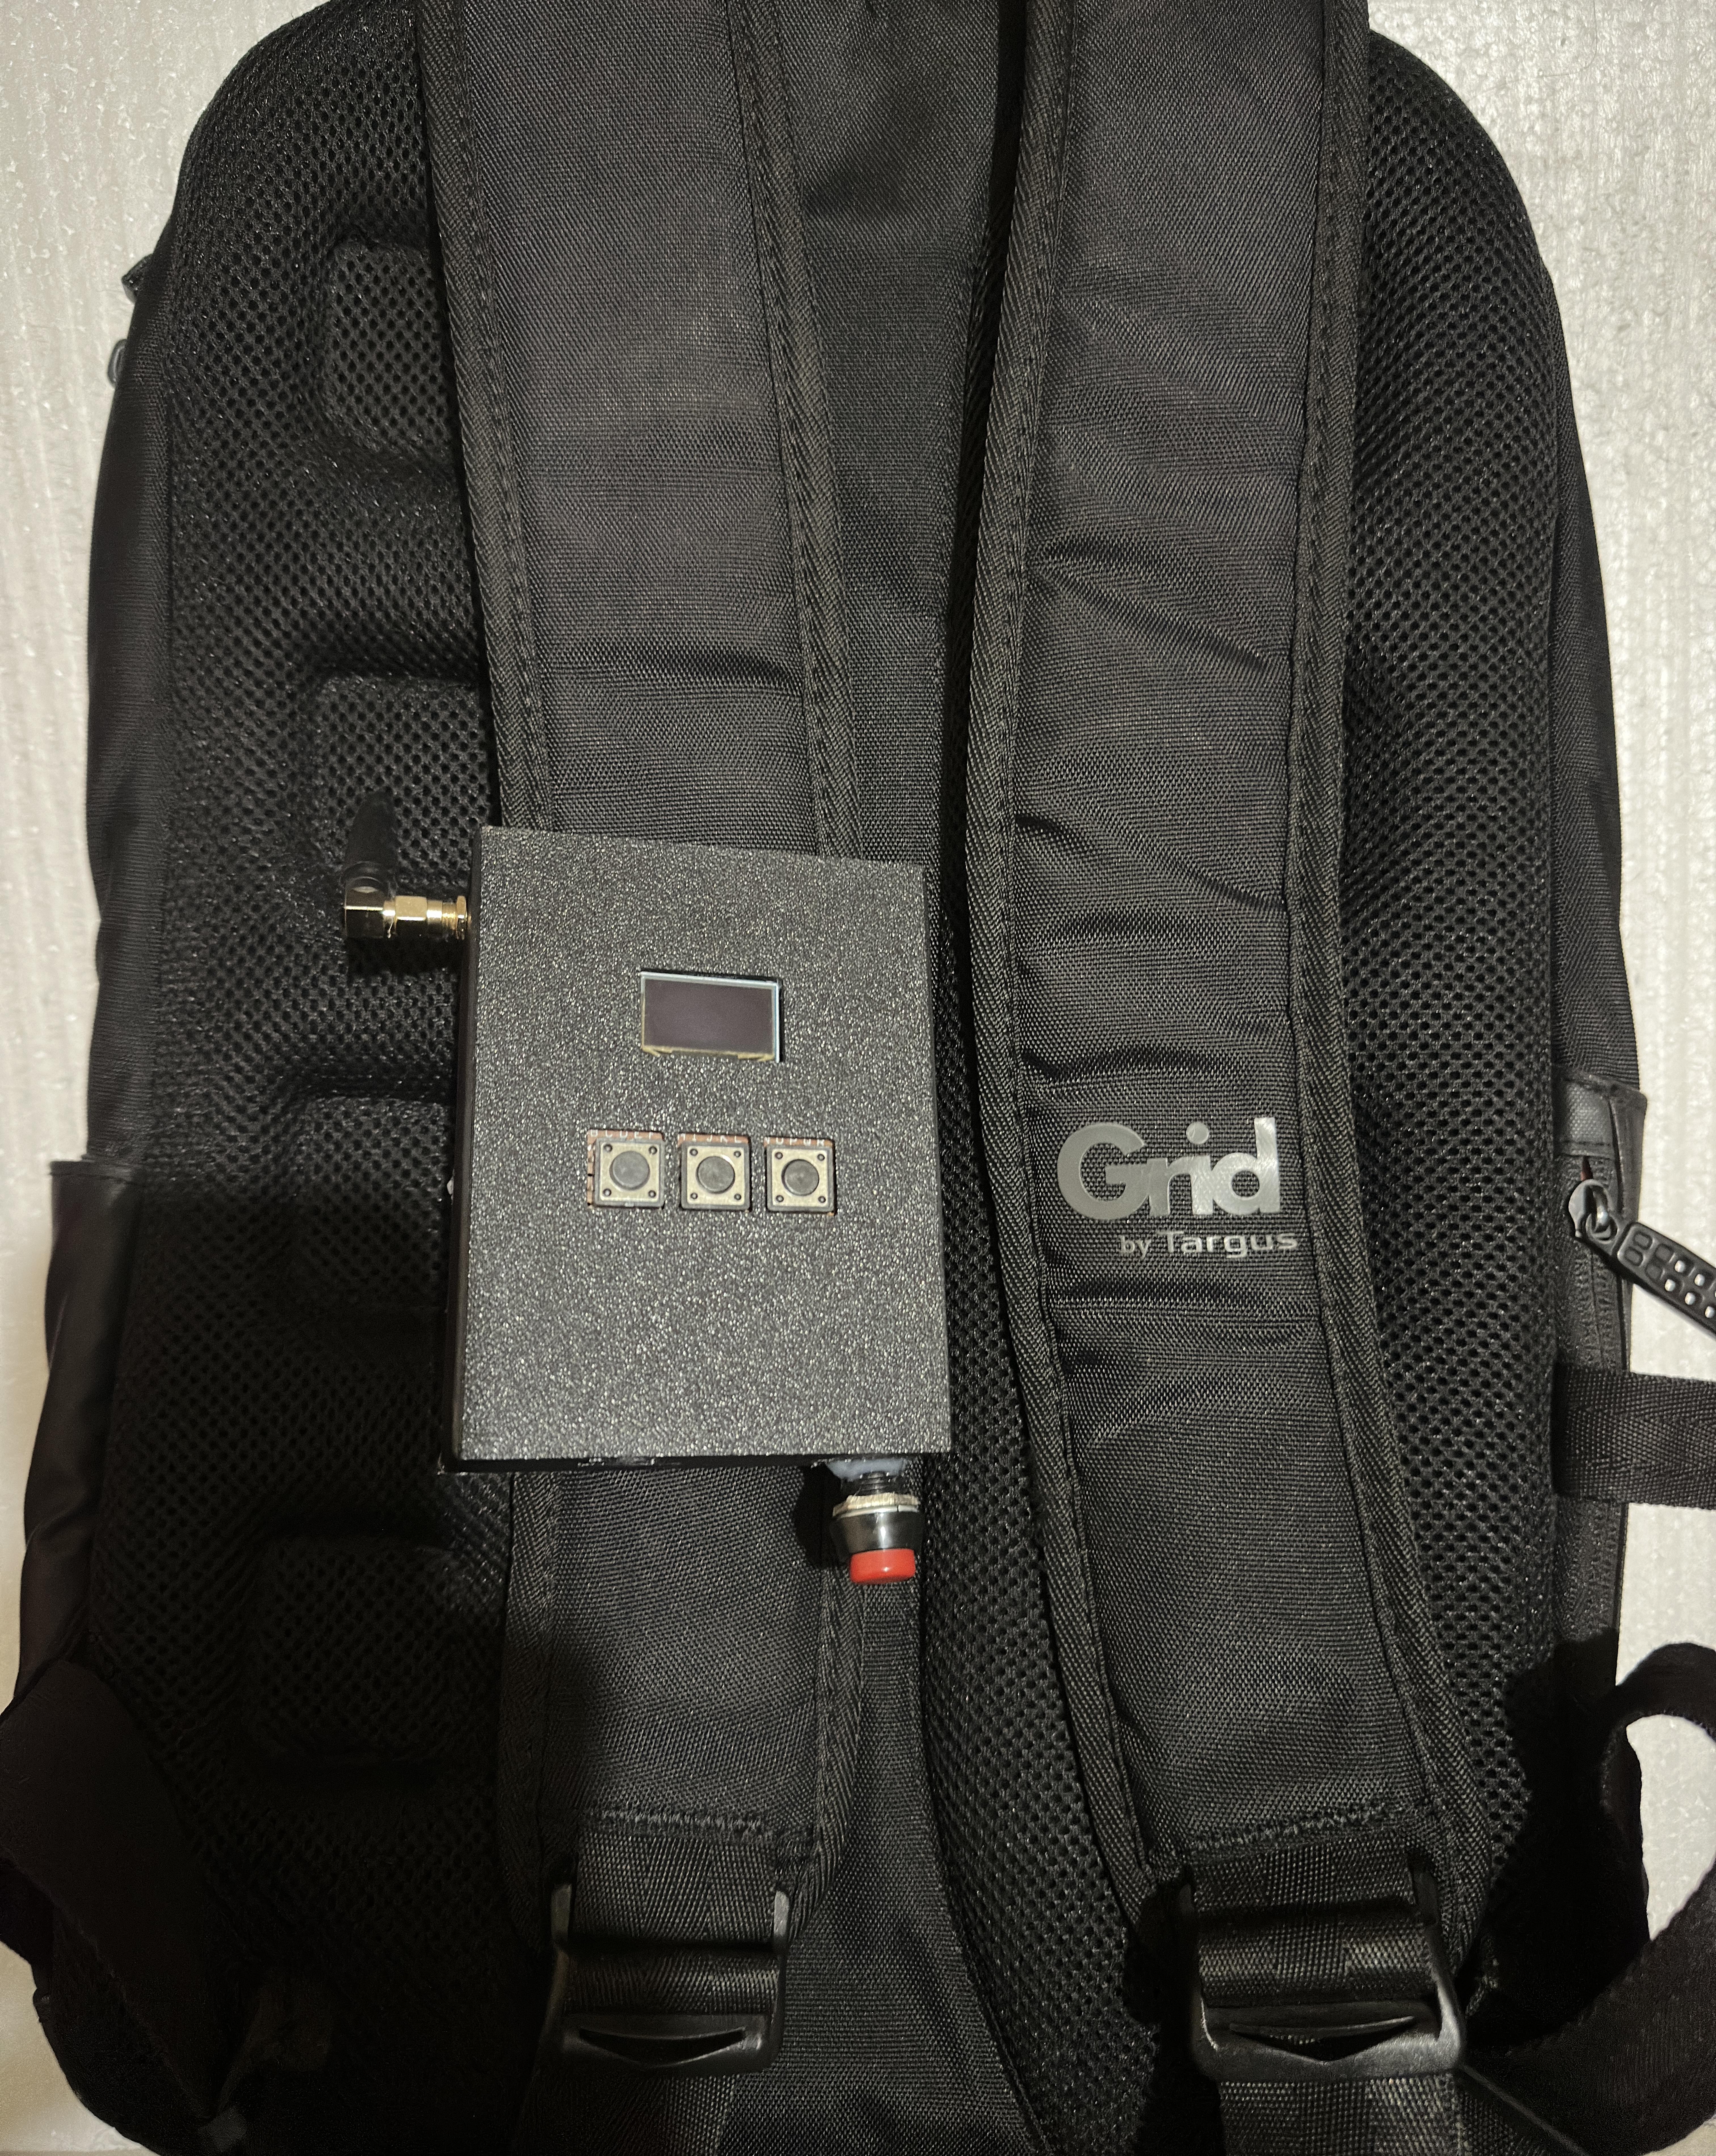
\includegraphics[width=0.6\textwidth]{figures/climber_mount.png}
    \caption{Demonstration of the Climber Main Device securely mounted on a backpack shoulder strap.}
    \label{fig:climber_mount}
\end{figure}

\section{Wristband Setup}
\begin{enumerate}
    \item Slide the device onto the elastic wrist strap.
    \item Fasten it securely around your wrist. The MAX30102 sensor window on the underside \textbf{must} be in direct contact with your skin, relatively tight to prevent ambient light leakage, but not so tight as to restrict blood flow.
    \item Turn on the device using the small side toggle switch.
\end{enumerate}

\begin{figure}[H]
    \centering
    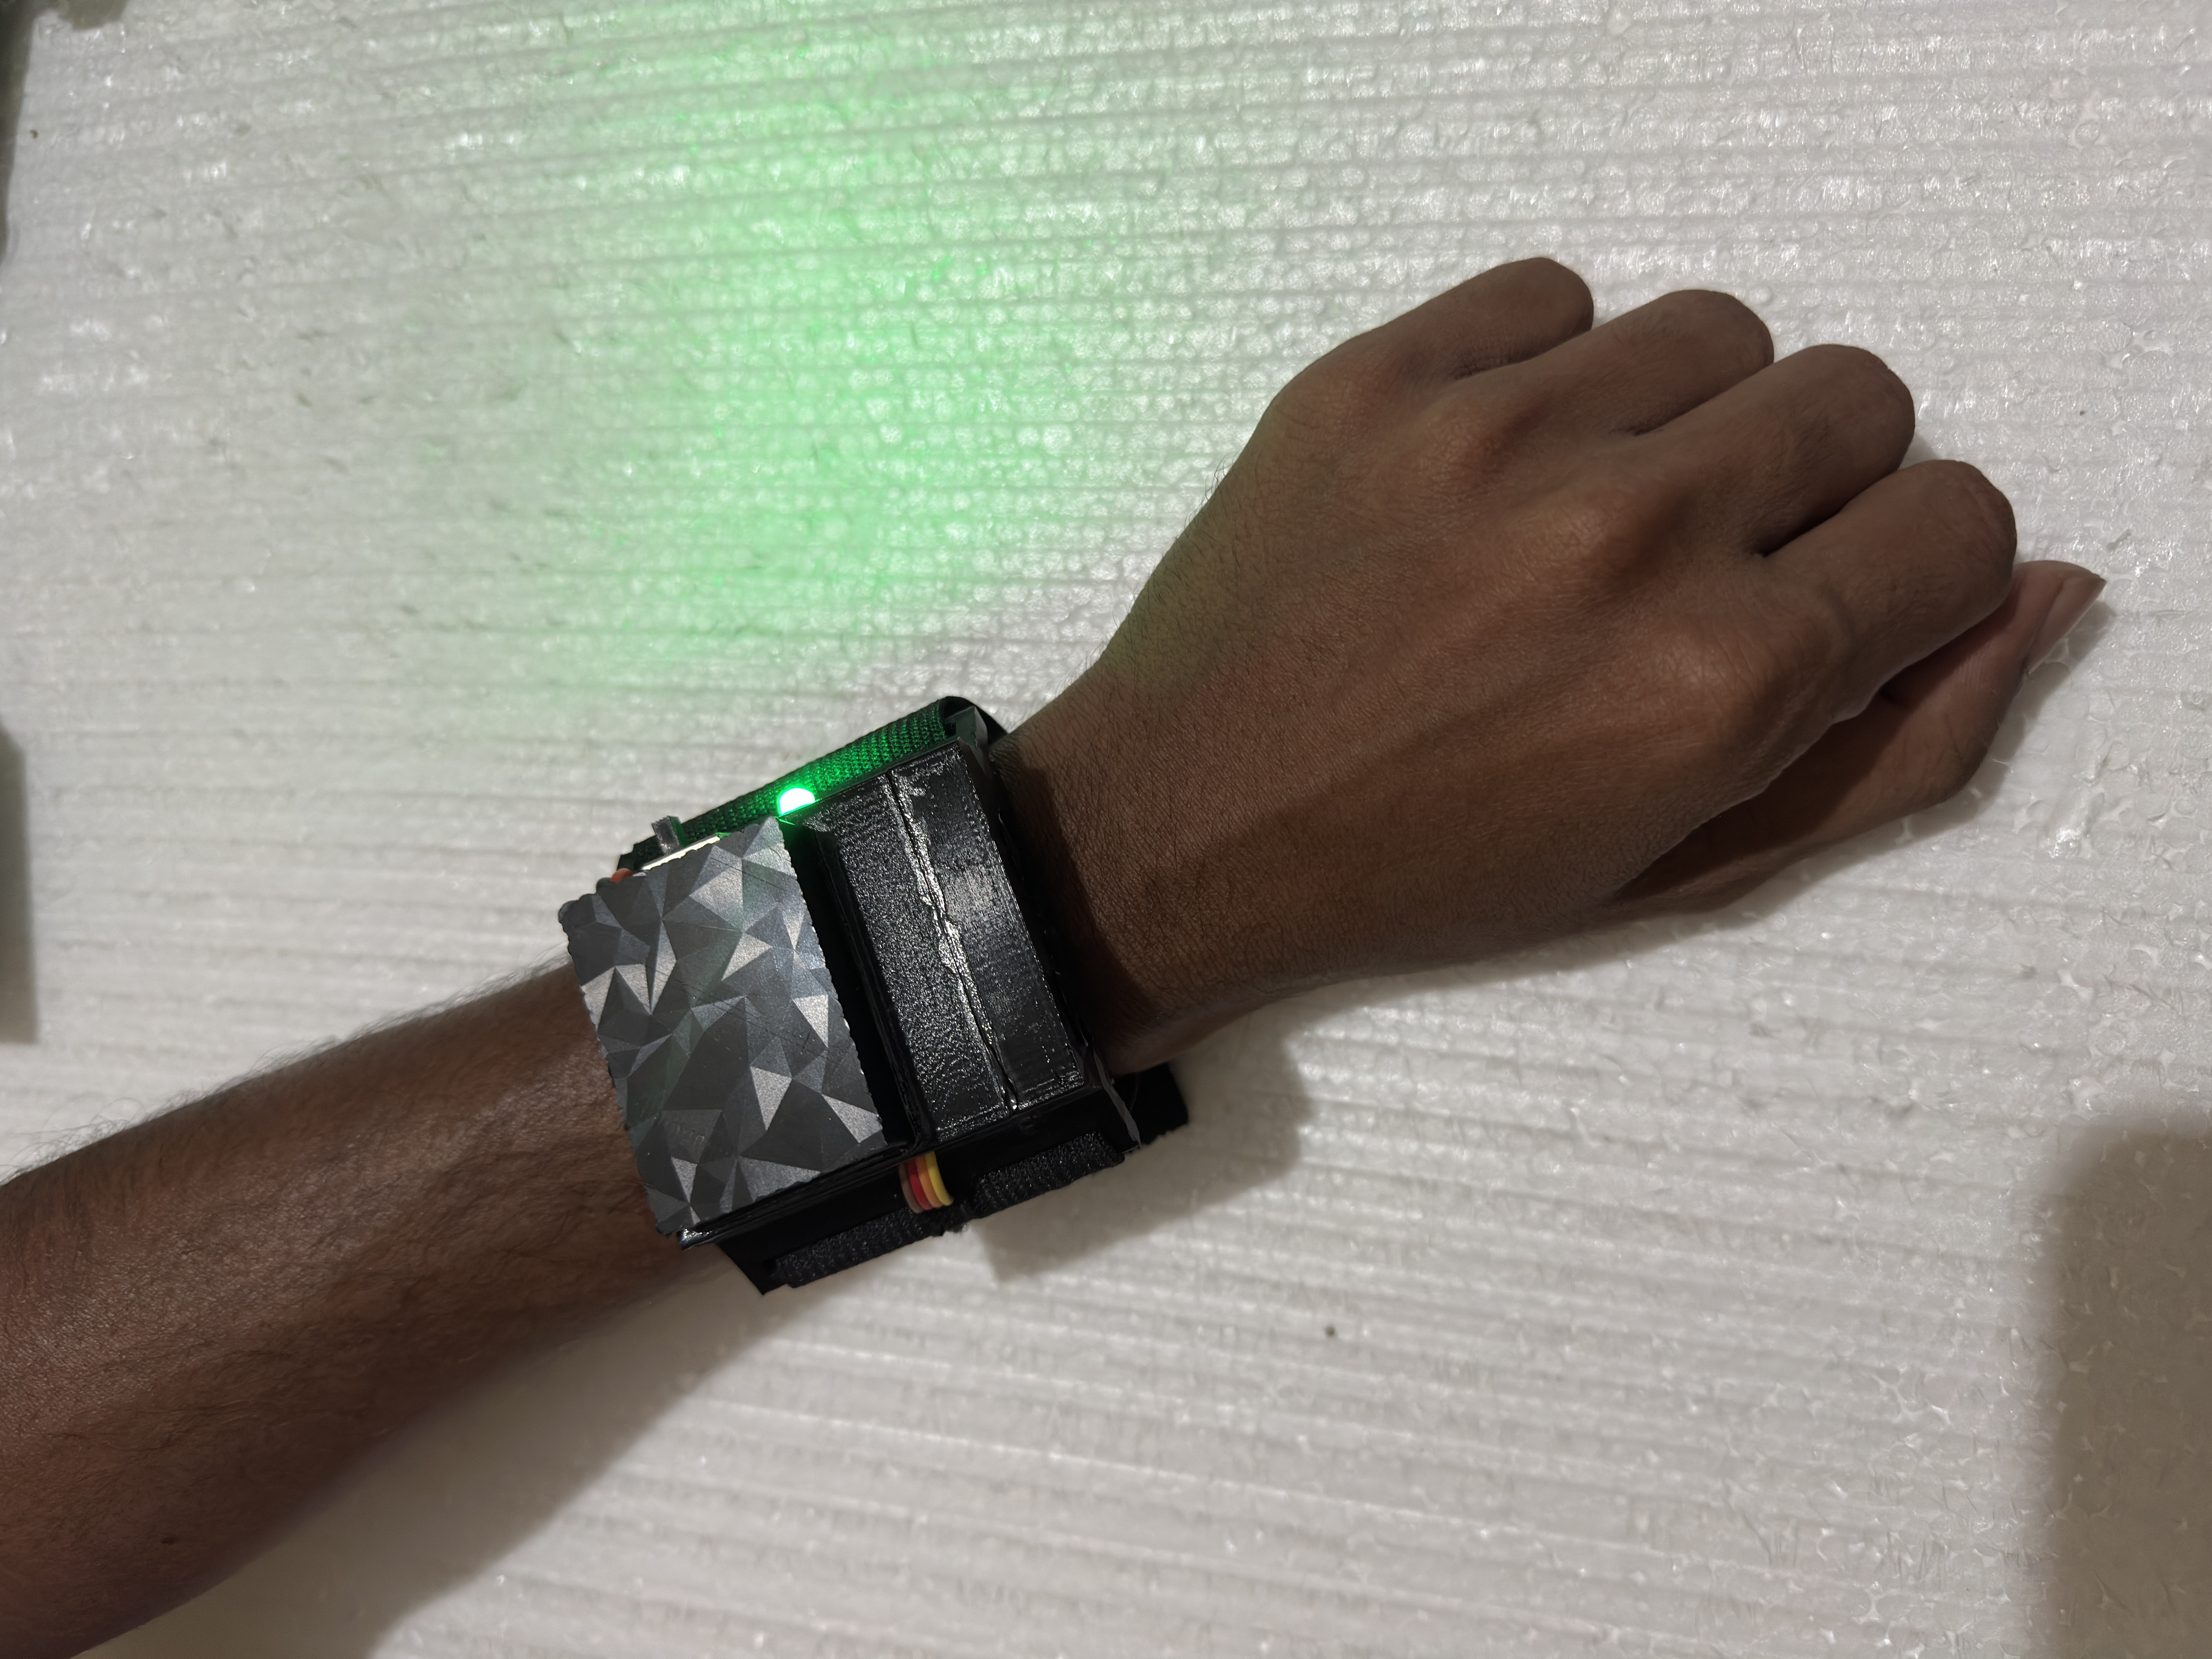
\includegraphics[width=0.6\textwidth]{figures/wristband_wear.png}
    \caption{Correct positioning of the wristband on the climber's arm.}
    \label{fig:wristband_wear}
\end{figure}

\section{Repeater Setup}
For the LoRa mesh network to function effectively, the Repeater must be placed strategically.

\begin{tipbox}
\textbf{Placement Strategy:} Place the repeater at a high elevation point with a clear line of sight to both the mountain trails and the base camp. Avoid placing it deep within ravines or immediately behind large metallic structures.
\end{tipbox}

\begin{enumerate}
    \item Arrive at the designated relay location.
    \item Power on the Repeater (hold power button for 3 seconds).
    \item Mount the device on a pole, branch, or rock using the straps, ensuring the LoRa antenna is oriented vertically.
\end{enumerate}

\section{Base Camp Unit Setup}
The Base Camp unit connects the local LoRa network to your monitoring dashboard.

\begin{enumerate}
    \item Place the Base Camp Unit on a stable surface near the monitoring laptop, preferably near a window or outside the tent for better LoRa reception.
    \item Connect the Base Camp Unit to the laptop using the provided USB data cable.
    \item Power on the device.
    \item Open your laptop's Device Manager or System Information to verify that the ESP32 is recognized as a COM port (Windows) or \texttt{/dev/ttyUSB} / \texttt{/dev/cu.SLAB\_USBtoUART} (macOS/Linux).
    \item Note the port name, as you will need to enter it into the Dashboard application (operating at 115200 baud).
\end{enumerate}

\begin{figure}[H]
    \centering
    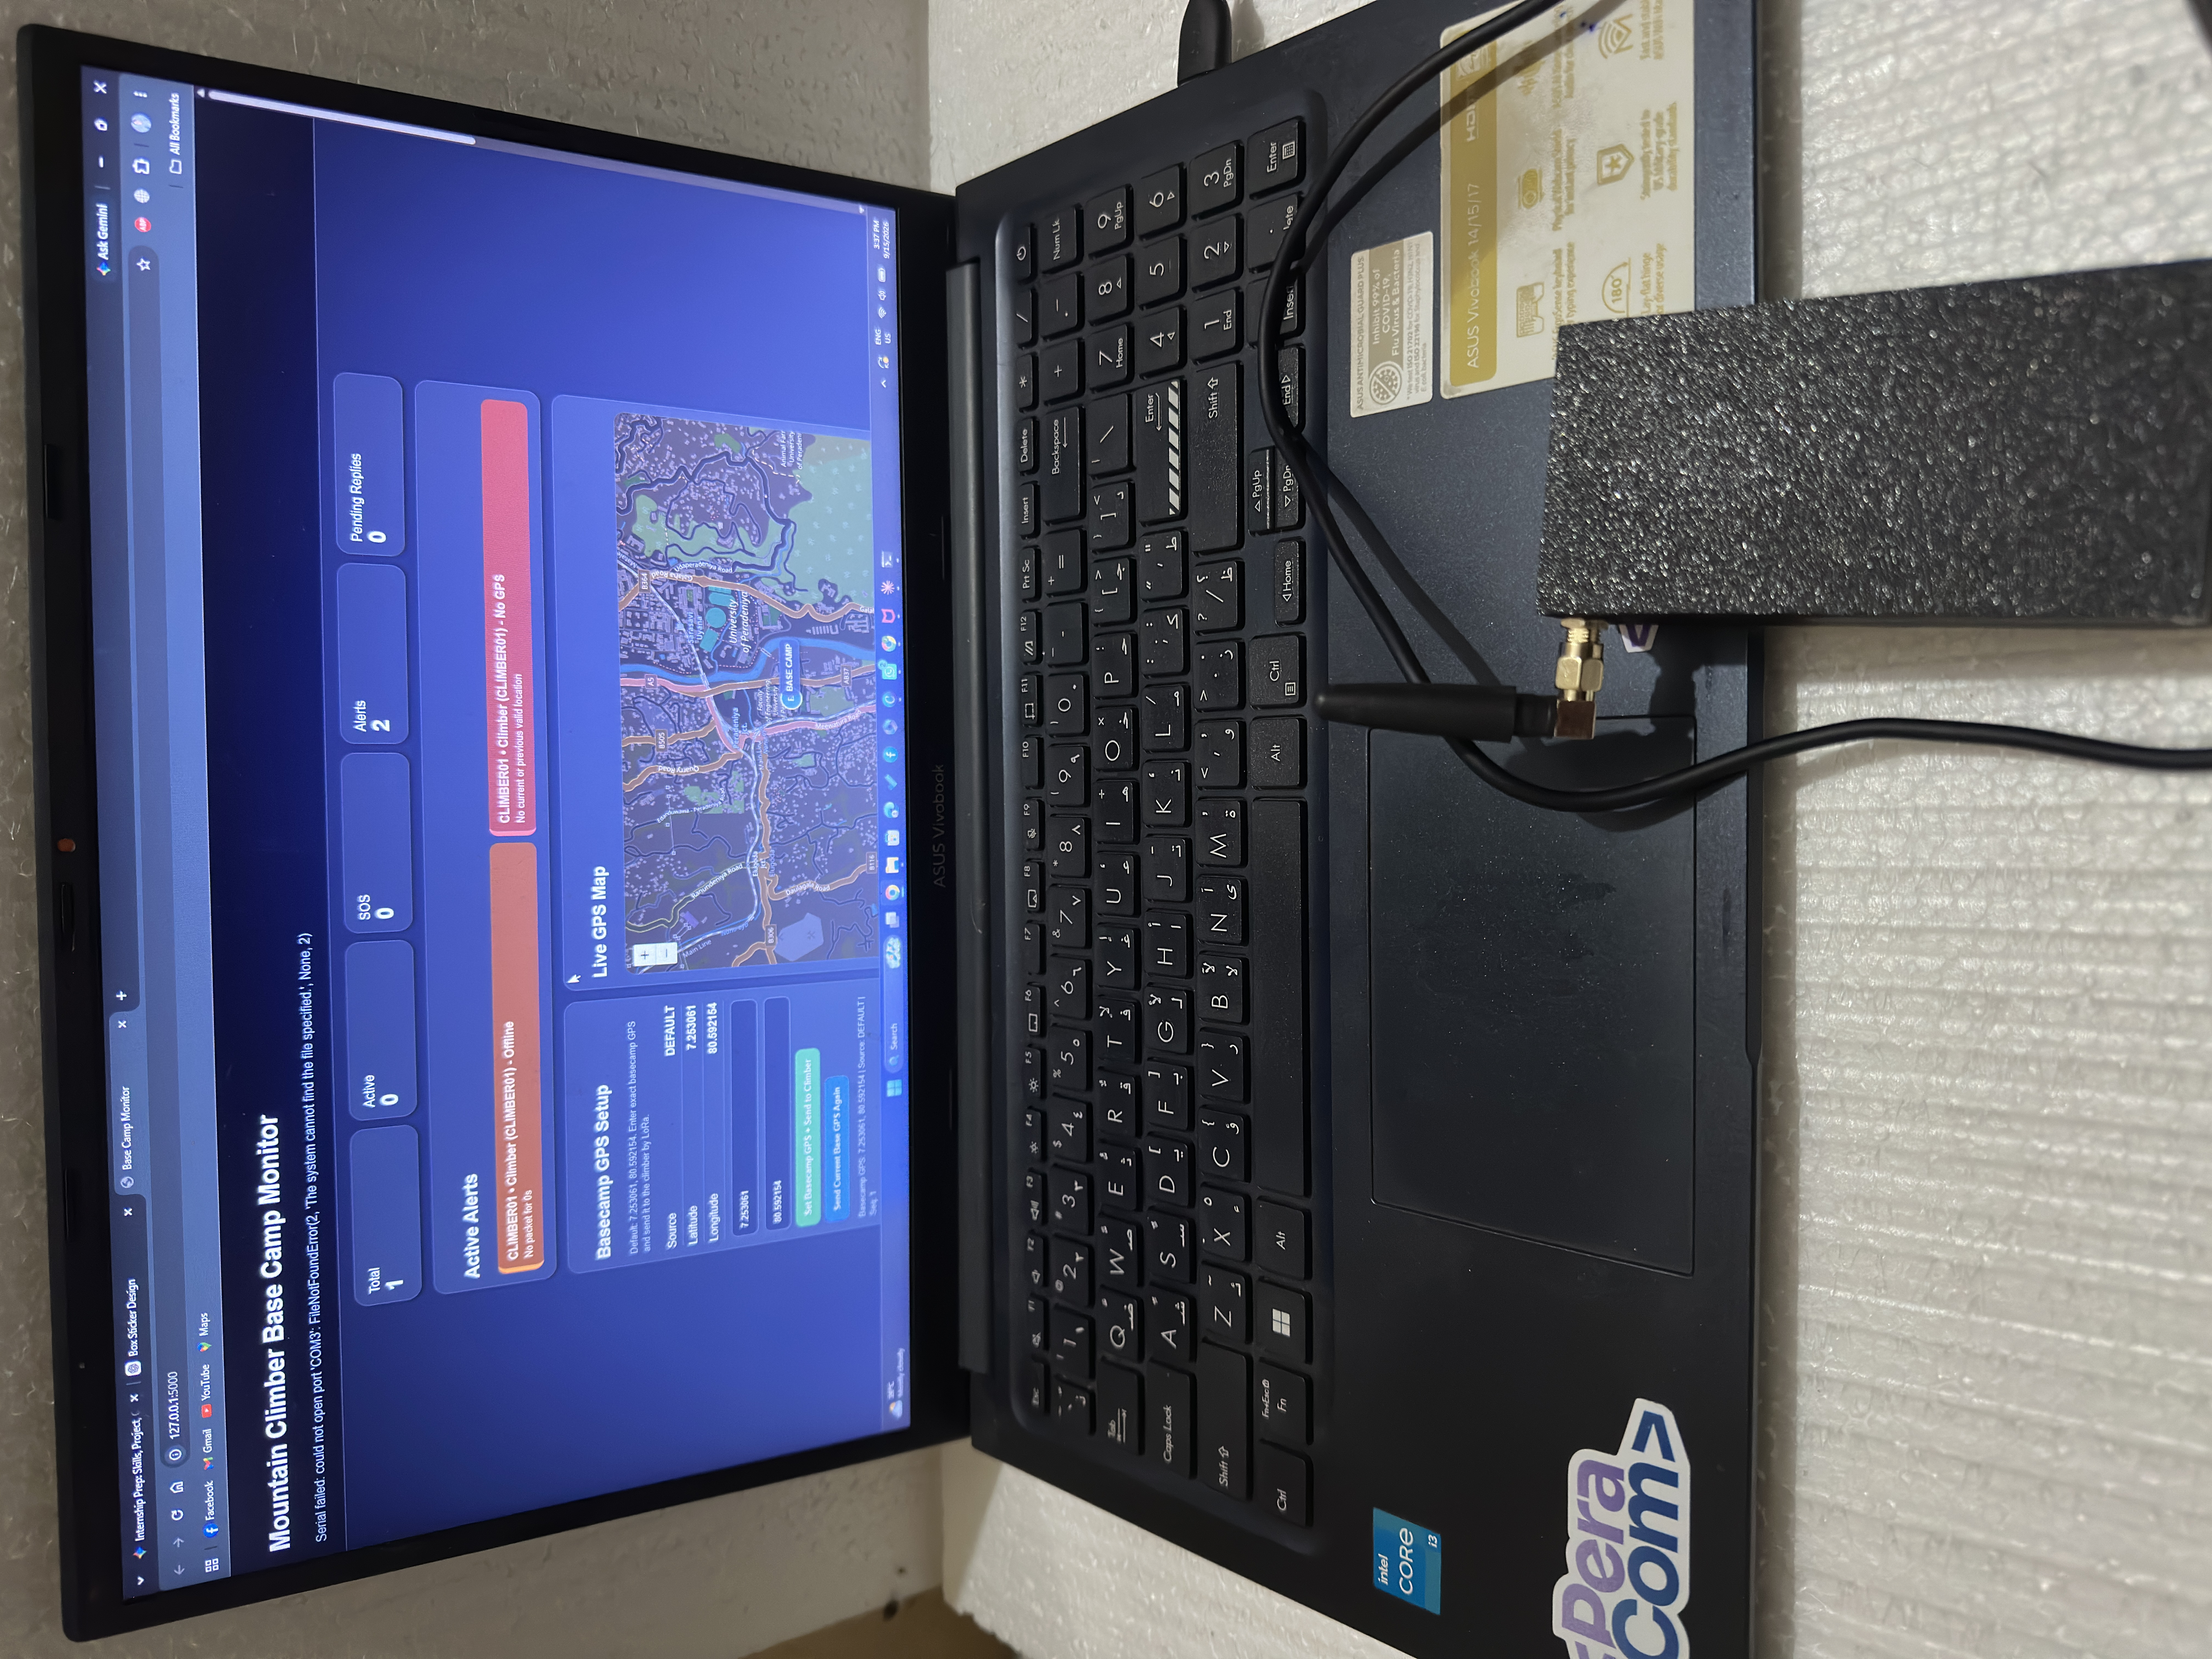
\includegraphics[width=0.7\textwidth]{figures/basecamp_setup.png}
    \caption{Base Camp Unit connected via USB to a laptop running the dashboard software.}
    \label{fig:basecamp_setup}
\end{figure}
